\chapter{绪论} \label{chapter:intro}

%\epigraph{... the ways by which men arrive at knowledge of the celestial things are hardly less wonderful than the nature of these things themselves}{\textit{Johannes Kepler}}

\section{引言}
\subsection{地球与人类,无独有偶?}

由古至今,人类在宇宙中的所处的位置就一直魂牵梦绕着人们的思绪。这个难题既
包括了人类居住的地球在空间上究竟是否独特,另一方面也包含人类(或生命)在宇
宙中的唯一性与否。而正因人类拥有了实证与思考的能力,因而在这个问题上的观测
与探索也从未曾停歇。

首先,行星科学(Planetology)是一门古老的以观测为基础的科学。早在公元前,古
希腊等各大文明已有天文学家(如伊巴谷)统计了相当可观的夜空发光天体的运行与
方位\cite{Xuan1992, wikipedia_astronomer}。而在以托勒密为代表所提倡的
地心说主导了这个星球一千多年后,文艺复兴时期的哥白尼等人也通过观测提出了日
心说\cite{Copernicus1543}。自此地球在空间位置谜团便开始层层被揭开,
地球的面貌(图 \ref{fig:rwalone})也愈发完整地展现在了人类面前。

\afterpage{
\begin{savenotes}
\begin{figure}[ht]
\centering
\begin{subfigure}[b]{.45\textwidth}
\captionsetup{width=0.9\textwidth}
\centering
\includegraphics[width=0.95\textwidth]{figures/chapter1/fig1a_Apollo17_BlueMarble.jpg}
\caption[Apollo 17 号船员拍摄的南半地球,拍摄时间 1972 年 12 月 7 日。(图片版权:NASA)]{Apollo 17 号船员拍摄的南半地球\footnotemark[1],拍摄日期为 1972 年 12 月 7 日。(图片版权:NASA)}
\label{fig:apollo17earth}
\setcounter{footnote}{1}
\addtocounter{footnote}{+0}\footnotetext{\url{https://www.nasa.gov/content/blue-marble-image-of-the-earth-from-apollo-17}}
\end{subfigure}
\begin{subfigure}[b]{.45\textwidth}
\captionsetup{width=0.9\textwidth}
\centering
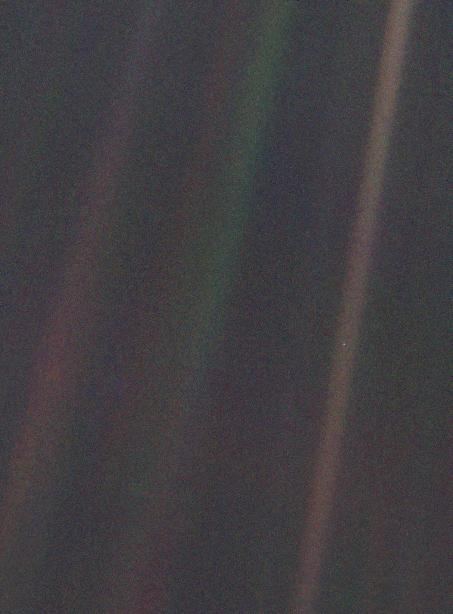
\includegraphics[width=0.95\textwidth]{figures/chapter1/fig1b_Voyager_PaleBlueDot.jpg}
\caption[Voyager 1 于 1996 年 9 月 12 日拍摄到的多色合成地球肖像照。(图片版权:NASA/JPL-Caltech)]{Voyager 1 于 1996 年 9 月 12 日拍摄到的多色合成地球肖像照\footnotemark[2]。(图片版权:NASA/JPL-Caltech)}
\label{fig:voyagerearth}
\addtocounter{footnote}{+1}\footnotetext{\url{http://photojournal.jpl.nasa.gov/catalog/PIA00452}}
\end{subfigure}
\caption{人类从太空看到的赖以居住和生存的母亲行星 --- 地球。\textbf{(a)} Apollo 17 号飞船航向月球的途中宇航员们回望并拍摄到的地球。这张图被称作「蓝宝石」,图中可以清晰的看到南半球的大气云层与被冰雪覆盖的南极点,另外还可看到非洲与亚洲大陆。\textbf{(b)} Voyager 1 航天器在距离太阳四十亿公里外拍摄到的地球。在最右侧的太阳散射光柱中,地球就只是不到一个像素的小白点,而在这颗蔚蓝的星球上曾居住并流逝着所有的人类足迹。 }
\label{fig:rwalone} 
\end{figure}
\end{savenotes}
}

此外,人们往往会从哲学角度来思考地球与生命在宇宙中普遍与否。比如原子论的宇宙
描述早已开端于古希腊与古印度。随后,意大利哲学家 Bruno 亦于 1584 年提出无穷宇
宙论:太阳与地球在宇宙中并不特殊,不计其数的其他星体也和地球相差无几(文献\citen{Bruno1584})

\begin{quote}
Onde possiamo stimare che de stelle innumerabili sono altre tante lune, altre tanti globi terrestri, altre tanti mondi simili a questo.
\end{quote}

历史一脉相承至今,随着人们对太阳系内行星与地球的运动探求愈来愈充分,也许便不难
理解搜索系外行星与系外生命为何如此举足轻重。而且从技术层面上,人类也已经有足够
的能力将「第二颗地球」与「地外生命」放入可见的未来计划中\cite{WoolfAngel1998}。

\subsection{系外行星的定义}
    
二十一世纪以前,由于对冥王星的测量并不充分,科学界从传统层面上也似乎没有必要争
论如何去界定行星。尔后,随着更多的海外天体(Trans-Neptunian Objects,简称 TNOs)
被发现,冥王星是否还是太阳系第九大行星的争辩也愈演愈烈\cite{SternMitton2005}。
终于,国际天文学联合会(International Astronomical Union,简称 IAU)于 2006 年在
「B5 决议\footnotemark[3]」中给太阳系内的行星做出如下定义:
\setcounter{footnote}{3}
\footnotetext{\url{https://www.iau.org/static/resolutions/Resolution_GA26-5-6.pdf}}

\begin{enumerate}[leftmargin=1\parindent]
\item 必须拥有围绕太阳的轨道;
\item 质量应充分大,使得其自引力足够克服刚性力,以形成(近)球外形;
\item 另外,行星必须清空轨道临近的其它天体。
\end{enumerate}

根据此定义,冥王星不再属于行星范畴,而被称作一颗矮行星。那如今观测到的近 3500 颗
\footnote{来源 NASA Exoplanet Archive \url{http://exoplanetarchive.ipac.caltech.edu/index.html},数据库更新至 2017 年 2 月 14 日}
系外行星呢?从词源学上,行星(planet)一词取名自希腊语,那么系外行星(exoplanet)
自然也该遵循上述 2006-B5 决议。然而部分系外气态巨行星(Gas Giant)质量已经大于十
个木星质量($M_\tif{J}$),此类行星的质量上限在 IAU 决议中也并未给出。实际上,
早于冥王星争辩,IAU 系外行星工作小组就已规定真实质量小于 13 $M_\tif{J}$(或行星内
部氘元素热核反应的质量下限\cite{Baraffe2003})的行星才被称作系外行星\footnote{请查看链接
 \url{http://home.dtm.ciw.edu/users/boss/IAU/div3/wgesp/}}。在本文亦一律遵循以上两者来
定义系外行星。


\subsection{系外行星扼要史} 

人类从诞生之始就默默地注视着夜空的「神行者」--- 行星。而作为专注于研究系外行星系统
的科学(Exoplanetology),其研究对象则跳脱出传统可观测的太阳系各大行星,转向了银河
系内太阳周围临近的恒星。回顾历史,这门领域的兴起也并非一蹴即成,而是融入许多先人不
停探索、试错与更新的艰辛历程。

近代系外行星搜索开始于十九世纪中页,Jacob 在对 70 Ophiuchi 的天体测量数据中找到类似
行星的信号\cite{Jacob1855},然而 Moulton 后续观测立即证否了这颗行星\cite{Moulton1899}。
在随后的一个世纪内,对木星质量的系外行星探索逐渐变得活跃,如 van de Kamp 于 1963 年
将仪器系统信号误认为一颗围绕巴纳德恒星的行星(文献 \citen{vandeKamp1963})。

另外一面,Struve 在1952 年提出短周期类木系外行星可同时通过视向速度与测光探测的设想
\cite{Struve1952}。然而科学界当时理所应当都认为木星只能处在距离主星 5 AU 轨道上,因此
需要太长的时间跨度来确认探测\footnote{一般来说,由于引力所造成的周期信号被连续确认三
个周期以上便被认为是真实的天体信号。}。不过,恒星光谱学依然在其间飞速发展,HD 114762 
被发现拥有一颗非常接近系外行星质量上限的褐矮伴星\cite{Latham1989}。

此时,来自美国的二人团队 Wolszczan 和 Frail 于 1992 年利用射电脉冲信号的周期变化率在
脉冲星 PSR1257+12 周围率先成功探测到包含两颗约 3 $M_\oplus$ 行星的行星系统
\cite{WolszczanFrail1992}。而 Walker 等人则在对主序恒星长达 12 年的视向速度监测中,
宣布没有迹象表明他们嗅探到系外木星信号\cite{Walkeretal1995}。

同一年,来自瑞士日内瓦天文台的 Mayor 和 Queloz 做出了系外行星领域里程碑式的发现(文
献\citen{MayorQueloz1995}): 他们利用坐落在法国 Haute-Provence 天文台的 ELODIE 光谱
仪从 150 颗恒星样本中成功探测到第一颗类太阳恒星周围的行星  --- 51 Peg b(见图 
\ref{fig:51pegsi})。这颗轨道周期只有 4.23 天的类木行星于同一年被美国 Marcy 和 Butler 团
组证实,随后便引起了对此类行星(即热木星)形成理论机制广泛而又深远的讨论
(\S \ref{sec:pltfrmatntheory}),一直延续至今。

\begin{figure}[ht]
\centering
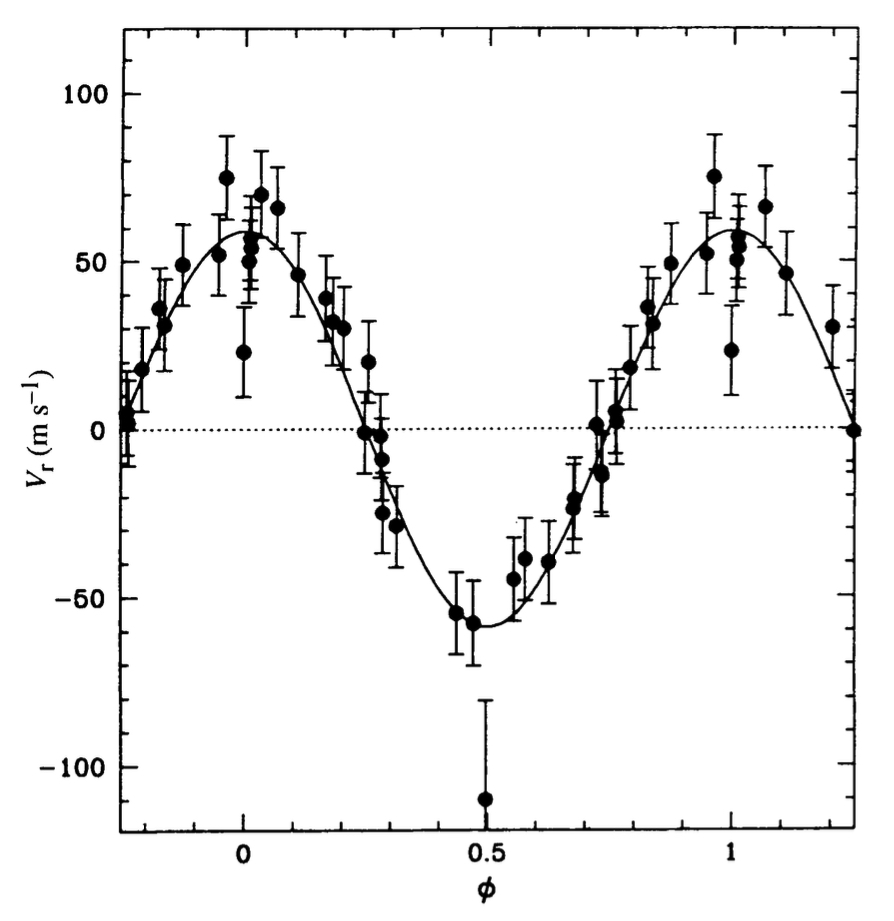
\includegraphics[width=0.95\textwidth]{figures/chapter1/fig2_51pegsi.jpg}
\caption[1995 年,日内瓦天文台天文学家 Mayor 和 Queloz 连续观测恒星 51 Pegsi 得到的视向速度曲线图,观测点已全数叠加至其伴星的周期 4.23 天。该系统主星是一颗类太阳恒星,因此视向速度曲线振幅所对应的最小质量为 0.47 $M_\tif{J}$ ,系人类首次发现到类太阳恒星周围的短周期类木行星。]{日内瓦天文台天文学家 Mayor 和 Queloz 连续观测恒星 51 Pegsi 得到的视向速度曲线图,观测点已全数叠加至其伴星的周期 4.23 天。该系统主星是一颗类太阳恒星,因此视向速度曲线振幅所对应的最小质量为 0.47 $M_\tif{J}$ ,系人类首次发现到类太阳恒星周围的短周期类木行星。图片取自他们于 1995 年发表在自然杂志的文献 \citen{MayorQueloz1995}。}
\label{fig:51pegsi}
\end{figure}

紧随其后的二十年内,系外行星领域各大新奇发现此起彼伏。图 \ref{fig:pltdiscyear} 为年度新
发现系外行星数目柱状图,该数目明显呈现出指数式增长,尤其是 2009 年 Kepler 太空望远
镜\cite{Boruckietal2010} 的发射新带来了大批通过凌星法发现的系外行星。图\ref{fig:pltdiscyear} 
中所展现的愈加多样化的样本也极大地丰富了我们对系外行星的认知。

\begin{figure}[hb]
\centering
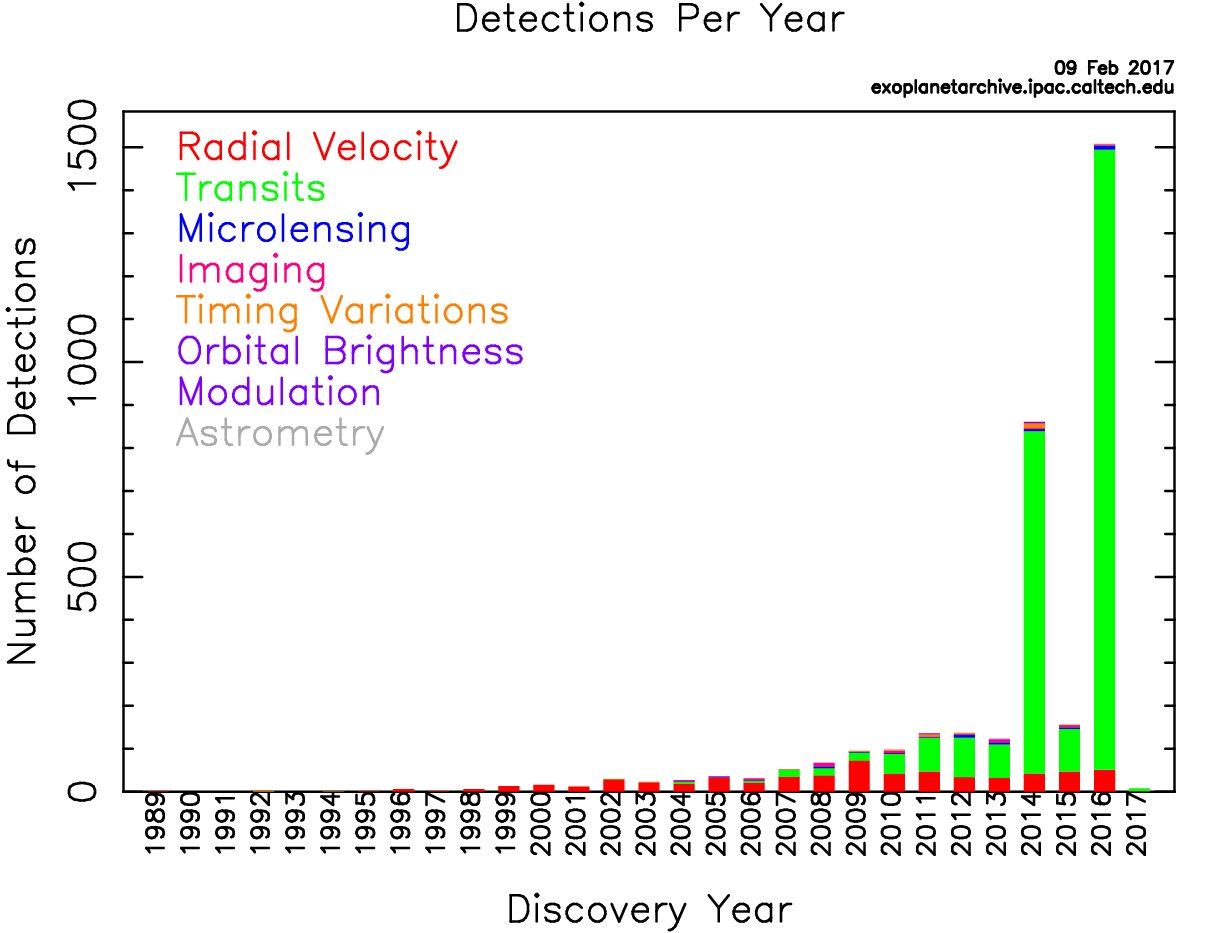
\includegraphics[width=0.95\textwidth]{figures/chapter1/fig3_nasaexo_dischist.jpg}
\caption{系外行星发现数量趋势图,不同颜色代表不同的探测方法(参照 \S \ref{sec:detmeth}),可以看出该数目呈现指数式增长。(图片取自 NASA Exoplanet Archive)}
\label{fig:pltdiscyear}
\end{figure}



\section{探测方法} \label{sec:detmeth}

天文学所研究的天体普遍离地球遥远,因而观测手段也主要集中在分析天体发射的光子上。
观测系外行星相较与恒星或太阳系内行星,通常要求非常高分辨率、灵敏度和稳定性的仪器,
也因而会遇到诸多困难,甚至还得排除恒星自身活动的干扰。比如测量围绕类太阳的系外地球
需要精度为 1 m s$^{-1}$的视向速度测量,相当于使用分辨率为 R = 100,000 的光谱仪器探测
主星光谱约 $10^{-6} \AA$ 的移动大小。参考书籍 \citen{Perryman2014exohb},本文亦大
致罗列目前探测系外行星主要方法如下:

\subsection{视向速度}

假使恒星周围存在行星,那么它们便会同时绕着公共的质心(COM)做开普勒运动。在观测中,这种三维运动可分解为视线平面内的二维运动与视线方向上的运动。视向速度(Radial Velocity,简称 RV)法就是通过测量视线方向上恒星谱线的多普勒红(蓝)移来探测周围行星的存在。

在简单的二体运动中,可以得到一颗轨道半长径为 $a$,质量为 $M_\tif{p}$ 的行星,可对质量为 $M_\tif{s}$ 的宿主恒星造成如下大小的半振幅视向速度 $K_1$(单位:米每秒):

\begin{equation}  \label{eq:rvk} 
K_1 \simeq \frac{28.4 }{\sqrt{1-e^2}} \frac{M_\tif{p}\sin i}{M_\tif{J}} \, \bigg(\frac{M_\tif{p}+M_\tif{s}}{M_\odot}\bigg)^{-1/2} \big(\frac{a}{1 \tif{AU}}\big)^{-1/2}
\end{equation}  %\myequations{视向速度法探测系外行星}


其中各物理量的意义参见附录\ref{apdx:twobodyproblem}。由上式可知,视向速度方法最重要的缺
陷即它只能测量(或拟合)出行星的最小质量(Minimum Mass,即$M_\tif{p}\sin i$)因为行星的轨
道倾角 $i$ 或视线方向夹角无法被测量。但与此同时,视向速度最明显优势是它可以精确测量行星
的轨道偏心率 $e$(图 \ref{fig:rvcurve} )。

\begin{figure}[h!]
\centering
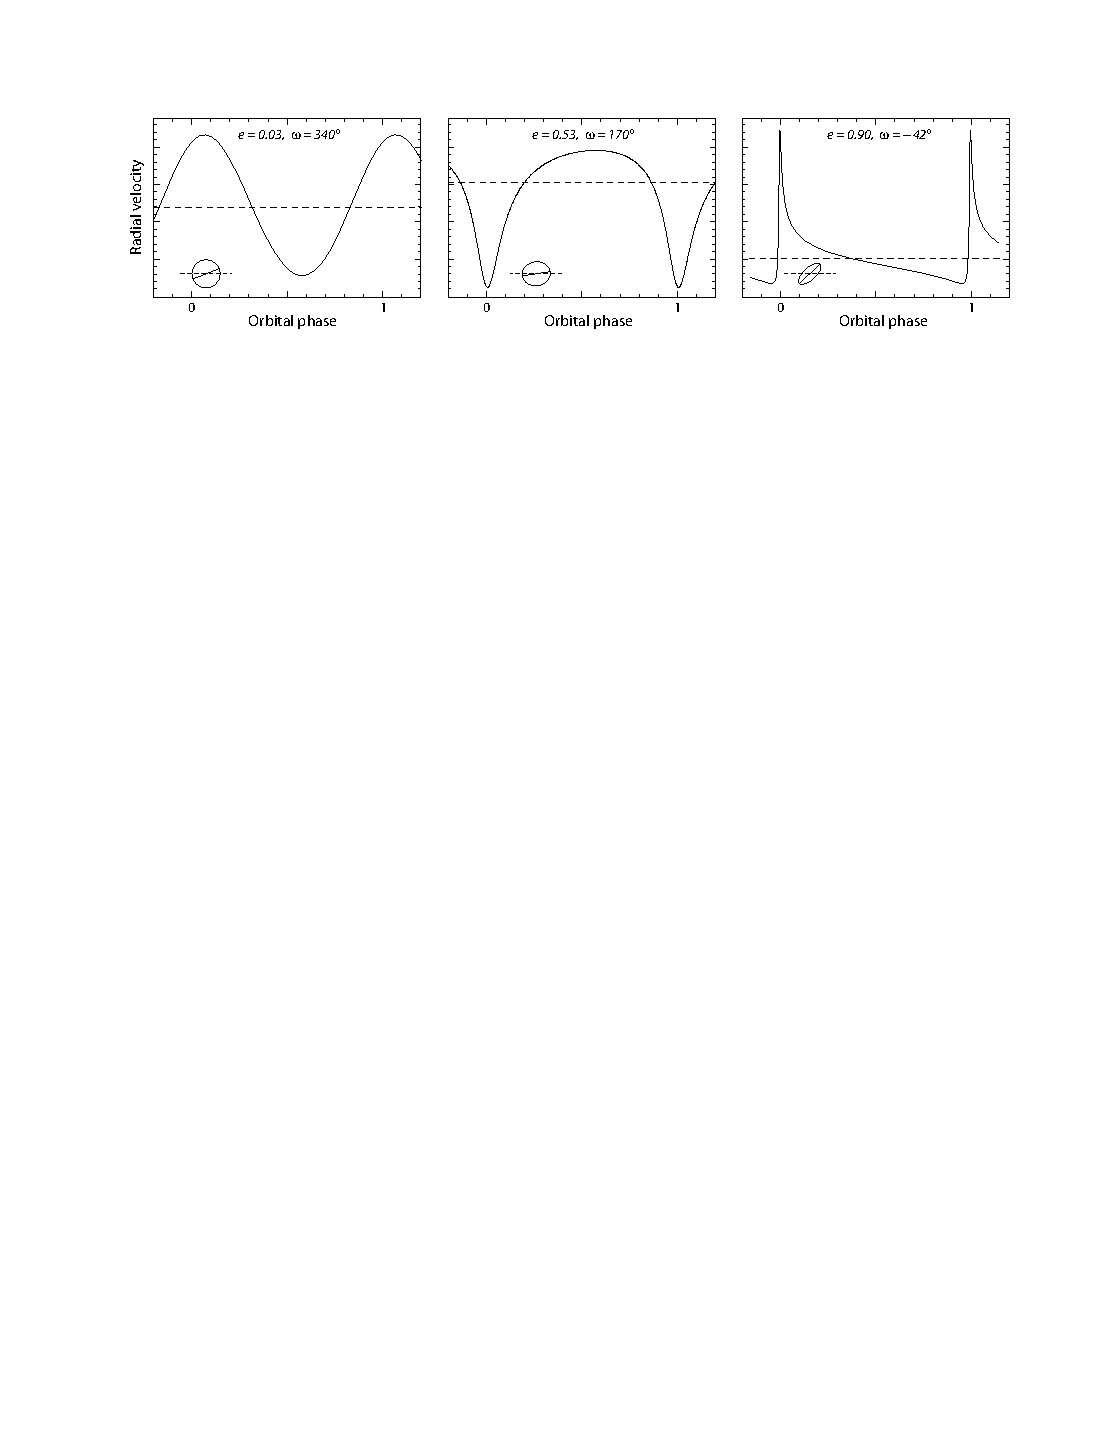
\includegraphics[width=1.0\textwidth]{figures/chapter1/fig5_rvcurve.pdf}
\caption[行星对主星造成的视向速度曲线示意图,从左至右分别代表不同的行星偏心率和轨道近心点取向。此图版权归 Perryman M. 所有。]{行星对主星造成的视向速度曲线示意图,分别代表不同的行星偏心率和轨道近心点取向。从左至右分别示意系统 HD 73256\cite{Udry2003HD73256},HD 142022\cite{Eggenberger2006HD142022} 和 HD 4113\cite{Tamuz2008HD4113}。此图取自文献 \citen{Perryman2014}。}
\label{fig:rvcurve}
\end{figure}

另外由于视向速度需要通过尽可能多的主星谱线来确认谱线的位移,因而往往更容易探测到 FGKM 型
主序星附近的大质量行星。在这里值得一提的是,由 Murphy 等人提出的激光频率梳法\cite{Murphyetal2007lasercomb}
与 Molecule Iodine Cell 或 ThAr Lamps 等传统的光谱仪器定标方法相比,可以更稳定重复的覆盖同
样的谱线区间,因此未来在视向速度方法上有相当可观的应用前景。

%优缺点,国际主流望远镜和团队?

\subsection{凌星法}

从原理上来说,凌星法是通过测量行星遮挡主星时主星亮度(流量)的变化来探测行星的。如图 \ref{fig:transit} 所示,系外行星处于恒星与地球的连线时被称作凌星( Transit)或主掩食(Primary Eclipse),而当恒星处于系外行星与地球的连线时则被成为掩星(Occultation)或次掩食(Secondary Eclipse)\footnote{凌星被约定特指半径较小天体遮挡大天体,而掩星则相反。双星中的掩食通常只用于大小相近天体的互相遮挡}。

\begin{figure}[ht]
\centering
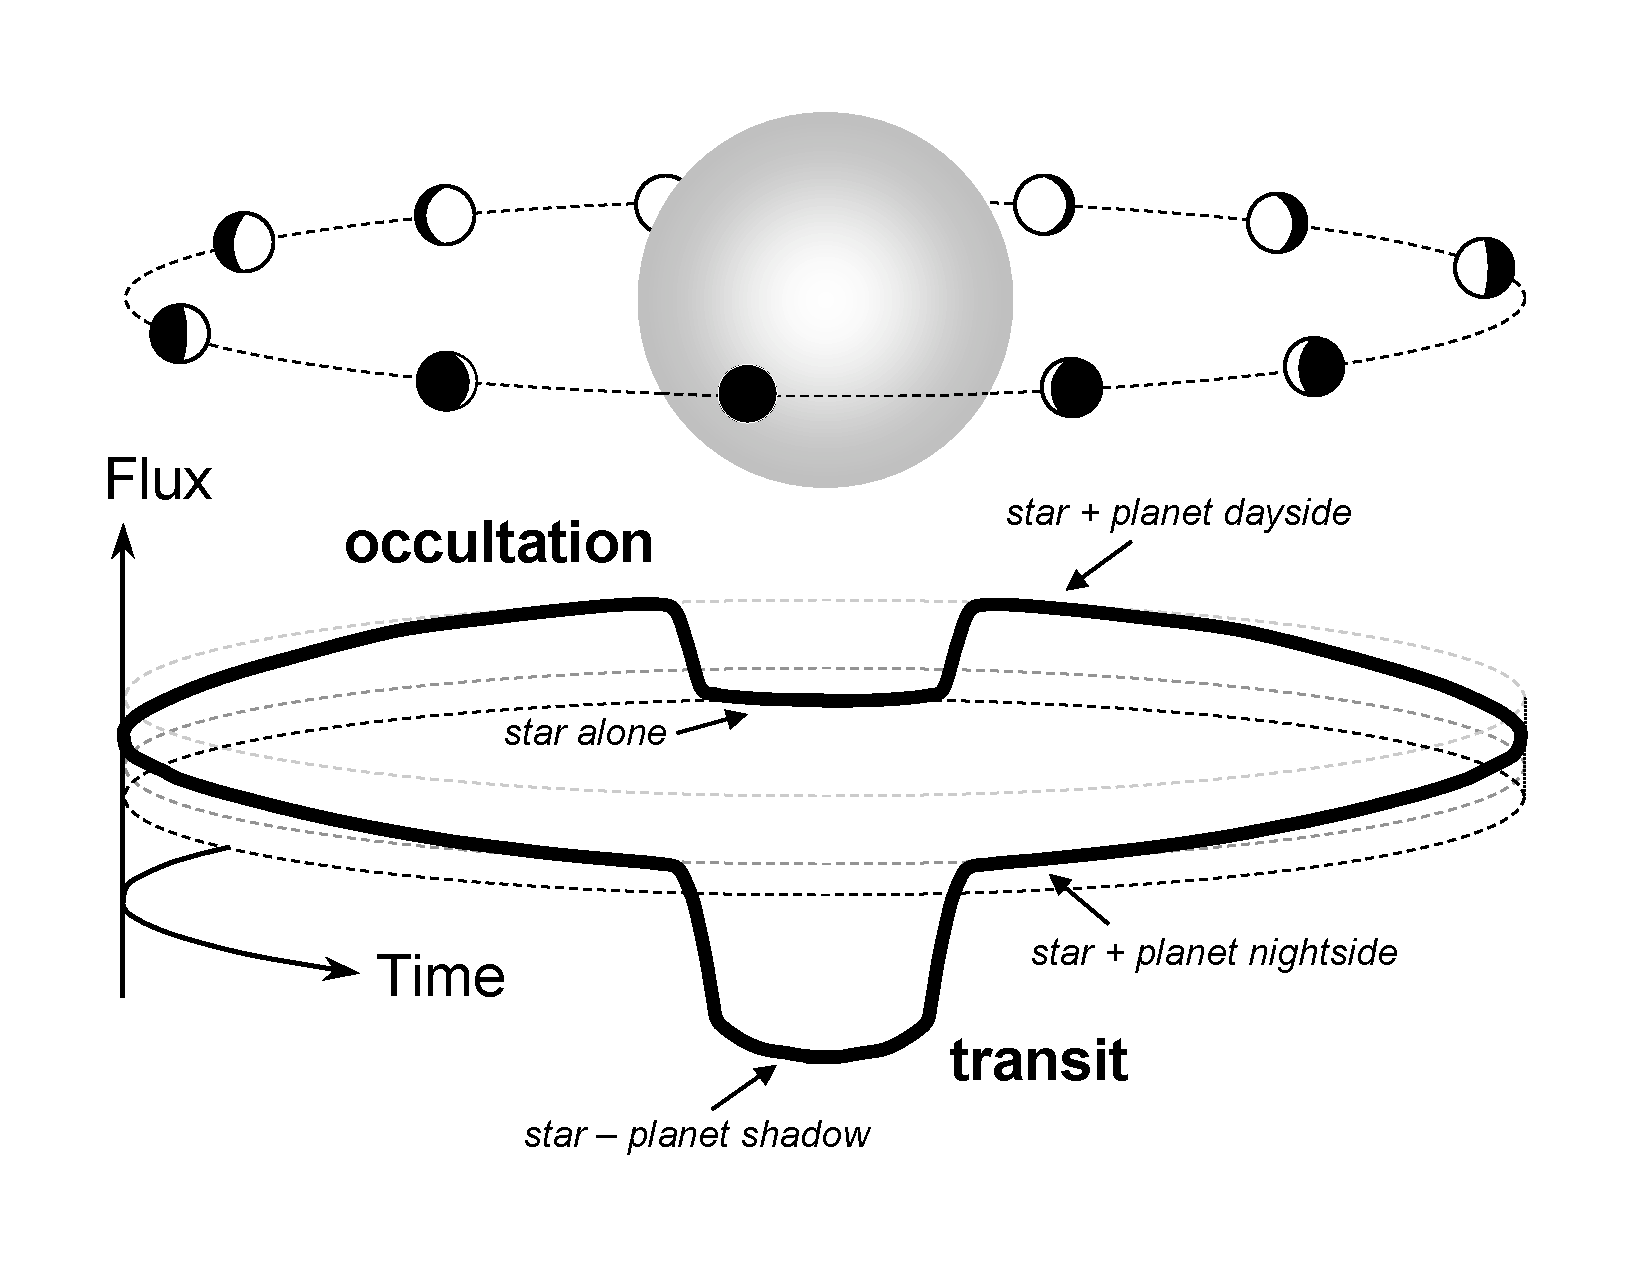
\includegraphics[width=0.95\textwidth,angle=-90, trim={0 1cm 0 0}, scale=0.9]{figures/chapter1/fig6_transit.pdf}
\caption[凌星法探测行星示意图,上半部分表示不同的轨道时刻。下方则为整个系统观测到的流量变化。版权 Joshua Winn。]{凌星法探测行星示意图,凌星法探测行星示意图,上半部分表示不同的轨道时刻。下方则为整个系统观测到的流量变化。此图取自书籍 \citen{Seager2010exobook}。}
\label{fig:transit}
\end{figure}

事实上,掩食在太阳系内已属屡见,比如日、月食和金星凌日现象。虽然凌星法探测与视向速度
法在原理上被 Struve 于同一年提出\cite{Struve1952},但真正意义上的第一次观测到系外凌星却
比视向速度晚了五年\cite{Seager2010exobook}。当时视向速度已经发现了 64 颗系外行星,在对
其中 6 颗行星系统的凌星监测中,行星 HD 209458 b 的主掩食成功被观测到\cite{Henryetal2000, Charbonneauetal2000}。
这种滞后主要是因为凌星发生的几何空间概率较低($p = R_\tif{s} / a$),与此同时还要求观测的
相对测光精度至少达到 5 \textperthousand(对应于木星凌太阳),凌星法也因此通常结合巡天计
划(尤其是大视场巡天)展开,因而提高测光精度、处理数据和去除假阳性信号也成了该方法的技
术难关\footnote{凌星法只能得到系外行星的候选体,一般还需额外使用其他方法联合认证该行星,如
中天时刻变化(Transit Timing Variation,简称 TTV)或者 RV。}。目前地面上比较成熟的巡天项
目,包括 The Trans-atlantic Exoplanet Survey(TrES)\cite{Alonsoetal2004TrES},XO
\cite{McCulloughetal2005XO},The Hungarian-made Automated Telescope Network(HAT)
\cite{Bakosetal2007HAT} 以及 Wide Angle Search for Planets(SuperWASP)
\cite{Pollaccoetal2006WASP},相应的空间巡天项目也有 Convection, Rotation and planetary 
Transits(CoRoT)\cite{Bargeetal2008CoRoT} 与 Kepler\cite{Boruckietal2010}。


\subsection{天体测量}

\begin{figure}[h!]
\centering
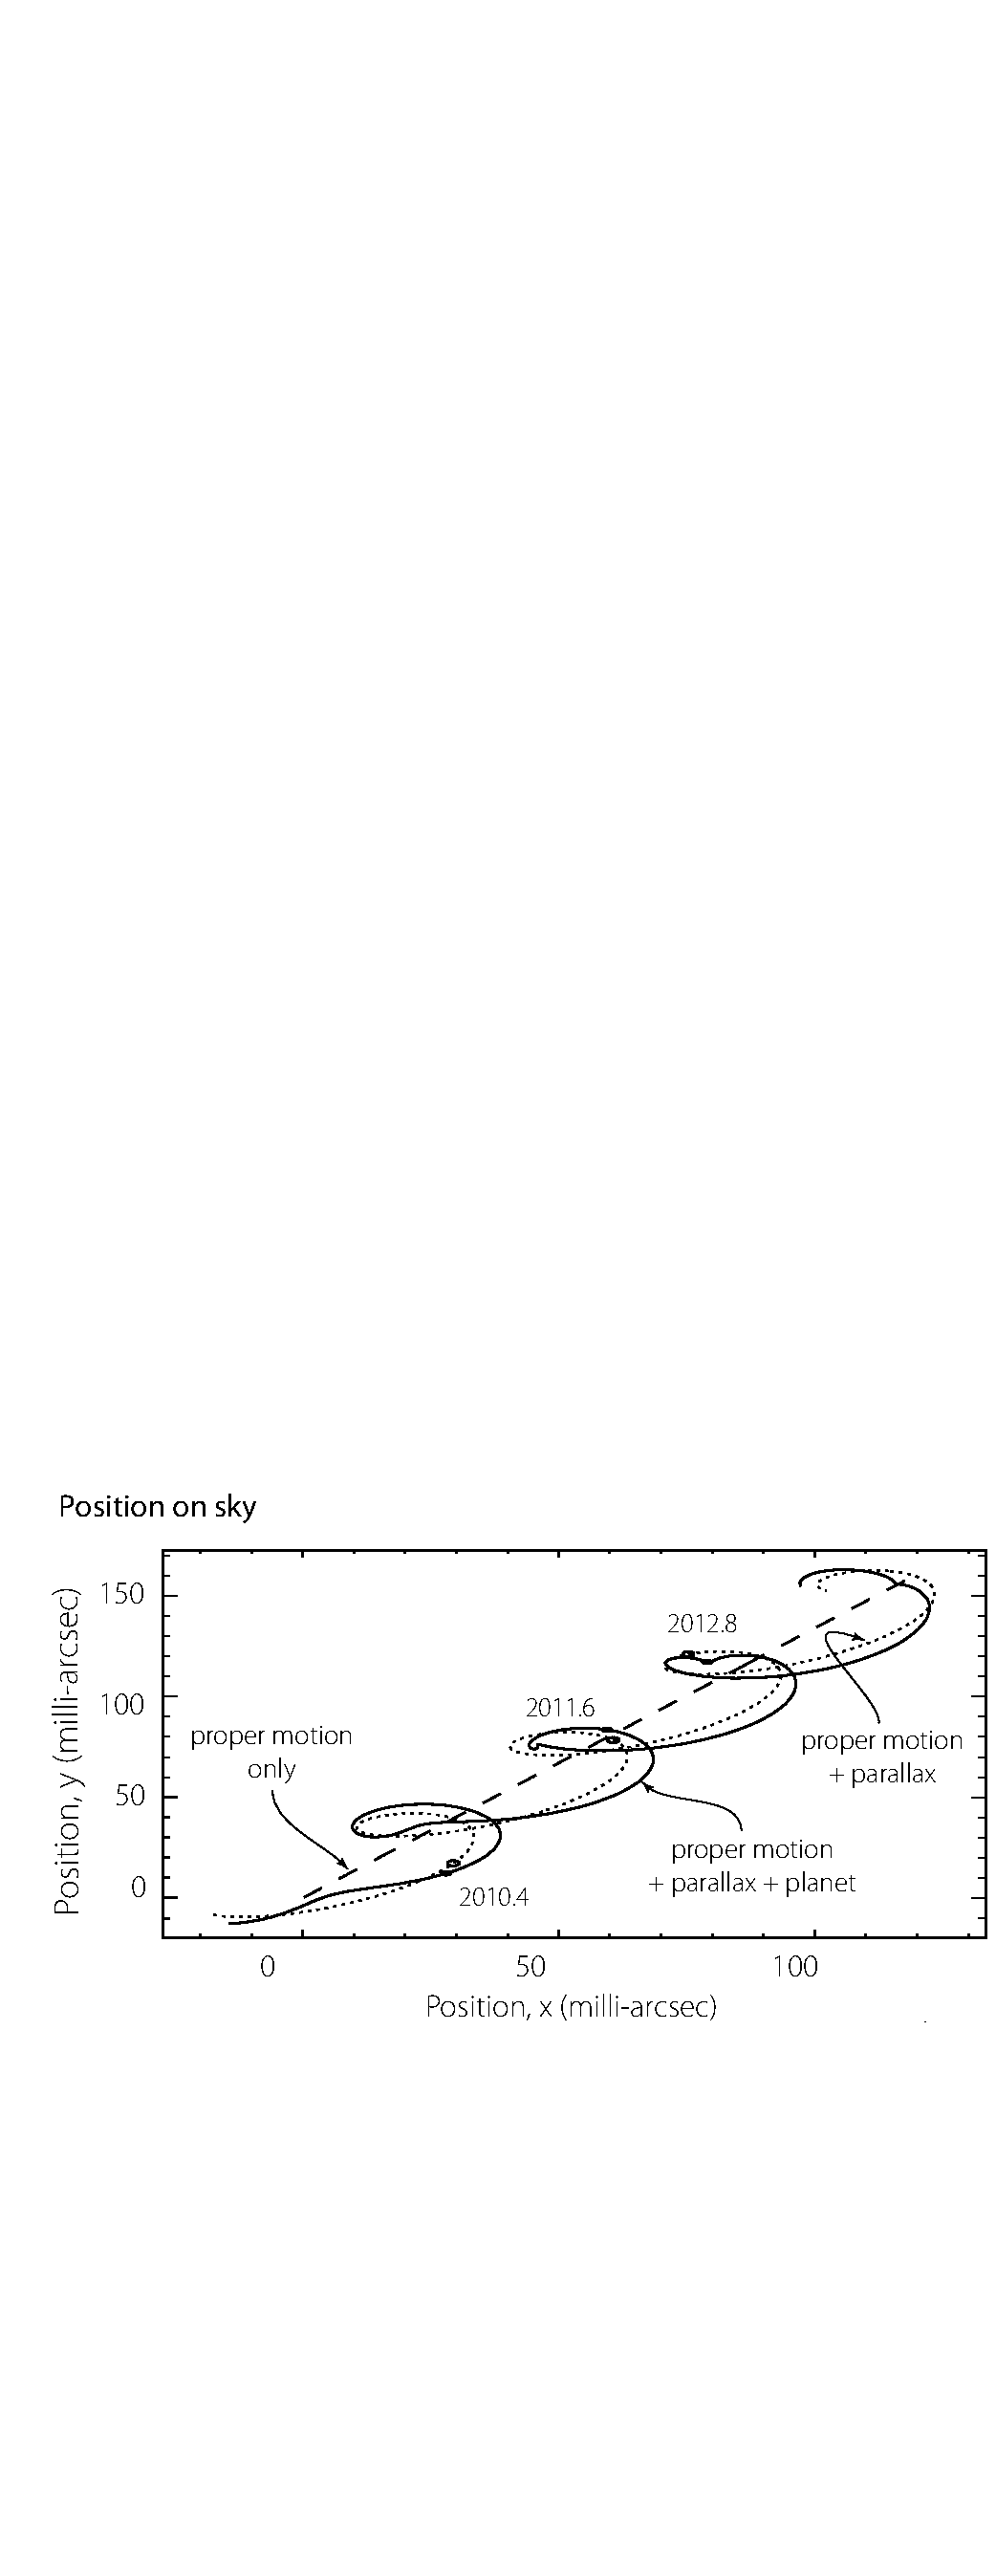
\includegraphics[width=0.95\textwidth]{figures/chapter1/fig7_astrometry.pdf}
\caption[由于行星的存在,宿主恒星的天球坐标随着时间的变化示意图,版权所有:Perryman M。]{由于行星的存在,宿主恒星的天球坐标随着时间的变化示意图。此图取自文献 \citen{Perryman2014}。}
\label{fig:astrometry}
\end{figure}

和视向速度探测主星前后摆动不同,天体测量法(Astrometry)着重于观测恒星在天球上的左右摆动。
行星对宿主恒星造成的来回振幅大小可用如下公式估算

\begin{equation}  \label{eq:astrometry} 
\alpha \simeq \bigg(\frac{M_\tif{p}}{M_\tif{s}}\bigg) \, \big(\frac{a}{1 \tif{AU}}\big) \, \bigg(\frac{d}{1 \tif{pc}}\bigg)^{-1} \tif{arcsec}
\end{equation} %\myequations{天体测量法探测系外行星}

如图 \ref{fig:astrometry} 所示,天体测量法只需要恒星在天球球面上的经度纬度信息就可探测到
行星,它也对主星的性质没有任何依赖,因而有其独特的优势,如可探测轨道倾角参数 $i$。
2013 年,Gaia 天体测量卫星成功发射,虽然目前来看科学数据尚未达到探测系外行星的精度
\cite{GaiaCo2016},期待今后几年会有振奋人心的成果。


\subsection{直接成像}
中国古话有道是「耳听为虚,眼见为实」,直接成像法便可把行星直观地展示出来。技术上这其实
并非易事:距太阳系几十个秒差距以外的行星与其主星的空间张角(Angular Separation)往往远
小于望远镜分辨率。即使空间上能分辨,恒星的黑体辐射也往往比行星高近十个量级(图 
\ref{fig:contrast})。在实际的观测中,对行星直接成像往往需要星冕仪(Coronagraph)或干涉仪
(Interferometer)的辅助(如图 \ref{fig:hr8799})。

\begin{figure}[h]
\centering
\begin{subfigure}[b]{.48\textwidth}
\captionsetup{width=0.9\textwidth}
\centering
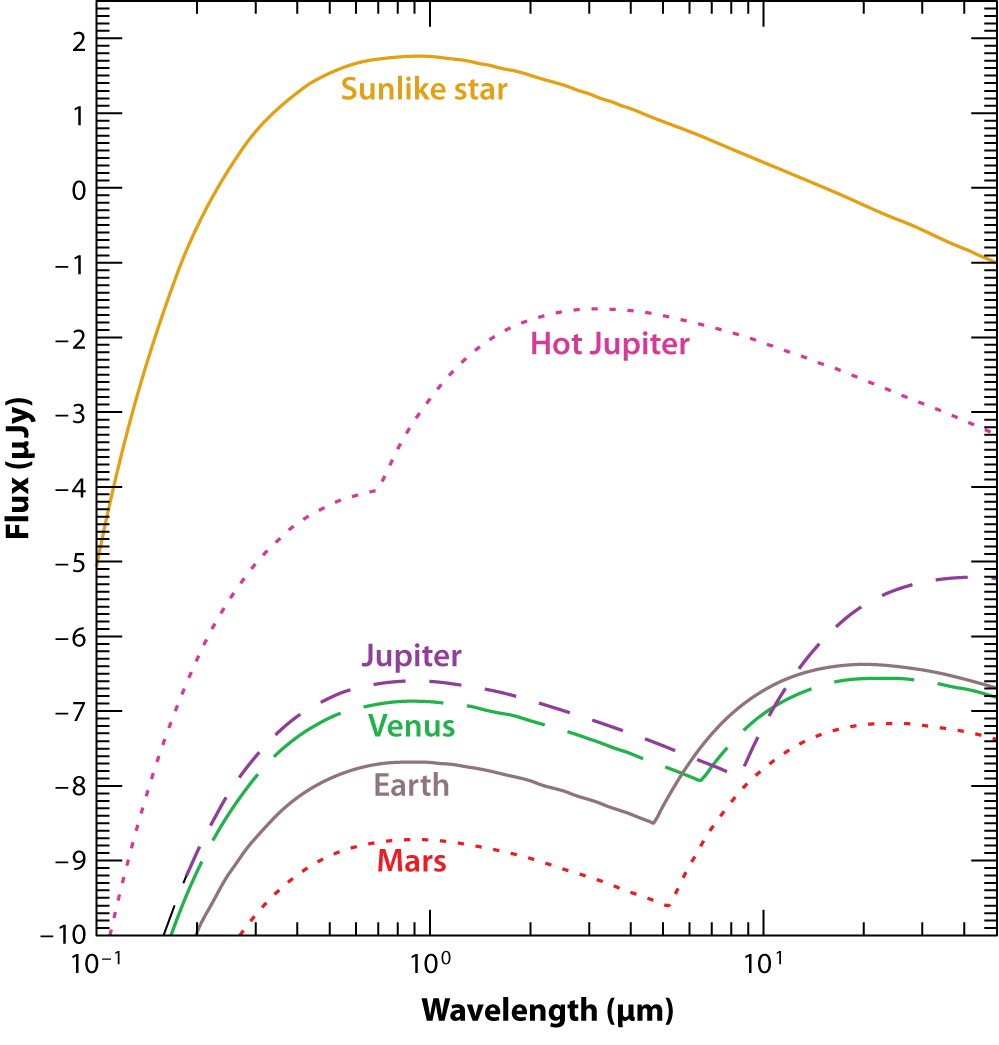
\includegraphics[width=0.95\textwidth]{figures/chapter1/fig8a_dicontrast.jpg}
\caption[仪器接受类太阳恒星在 10 pc 以外的黑体辐射(黄色实线),其余为太阳系行星与热木星在此恒星周围黑体发射与发射的叠加流量。在可见光波段行星与主星的对比度可差至十个量级,因此直接成像法一般选择在长波范围(如红外波段)探测系外行星。图片版权 Seager and Deming。]{可见光波段行星与主星的对比度可差至十个量级,因而直接成像法一般选择在长波范围(如红外波段)观测系外行星。图片摘自文献\citen{Seager2010}。}
\label{fig:contrast}
\end{subfigure}
\begin{subfigure}[b]{.48\textwidth}
\captionsetup{width=0.9\textwidth}
\centering
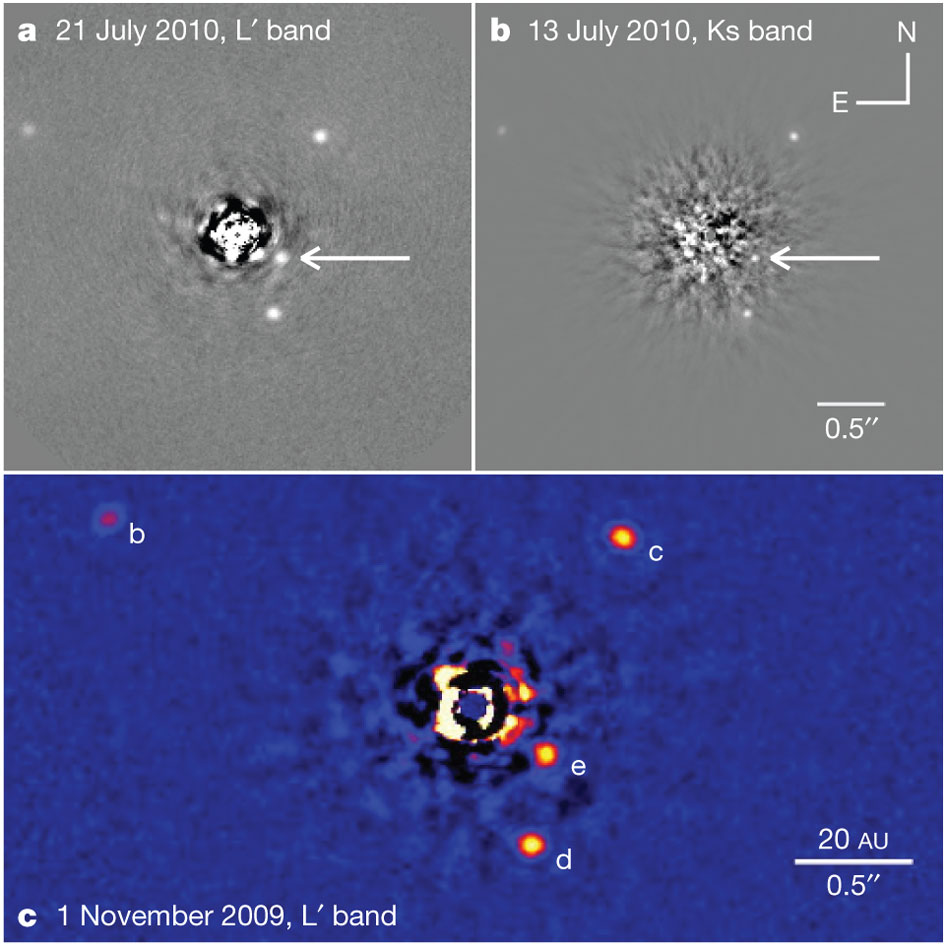
\includegraphics[width=0.95\textwidth]{figures/chapter1/fig8b_hr8799.jpg}
\caption[Keck 望远镜利用角向较差成像与自适应光学技术在近红外波段通过直接成像得到的 HR 8799 系统。中心恒星的大部分光已被星冕仪遮挡,留下小部分噪声,与远处四颗行星 。图片版权:Marois 等人。]{Keck 望远镜在近红外波段通过直接成像得到的 HR 8799 系统。中心恒星的大部分光已被星冕仪遮挡,留下小部分噪声,与远处四颗行星 。图片取自文献\citen{Marois2010}。}
\label{fig:hr8799}
\end{subfigure}
\caption{直接成像法探测系外行星。\textbf{(a)} 仪器接受类太阳恒星在 10 pc 以外的黑体辐射强度,其余为太阳系行星与热木星在此恒星周围黑体发射与发射的叠加流量。\textbf{(b)} Keck 望远镜利用角向较差与自适应光学技术直接成像观测到的 HR 8799 系统。}
\label{fig:directimage} 
\end{figure}

直接成像方法往往偏向于探测年轻的系统,如 HR 8799\cite{Marois2008HR8799}, 
Fomalhaut\cite{Kalas2008} 和 $\beta$ Pictoris\cite{Lagrange2010},这是因为行星在其形成早期会拥有较强
的近红外辐射。目前用于此方法的望远镜有 Hubble Space Telescope(HST),Keck,Very Large 
Telescope(VLT)和 Gemini Planet Imager(GPI)等\cite{Marois2008HR8799,Chauvin2005,Macintosh2014}。

\subsection{其他方法}
\textbf{微引力透镜(Microlensing):} 本方法原理可以追溯到 1936 年,Einstein 发表了一篇
计算前景星对视线方向上背景星引力放大率的文章\cite{Einstein1936}。而且在第一颗用微引力透镜观
测到的行星前,Mao 和  Paczynski 就已经从理论上提出了行星能在恒星引力透镜基础上造成额外的
微引力透镜效\cite{Mao1991}。如今已经有 42 个通过微引力透镜发现的系外行星系统,包括 2 个双行
星系统\footnote{参见 NASA Exoplanet Archive:\url{http://exoplanetarchive.ipac.caltech.edu/}}。在
役的仪器主要有 Optical Gravitational Lensing Experiment(OGLE)\cite{Udalskietal2002OGLE} 和 
Microlensing Observations in Astrophysics(MOA)\cite{Bond2004MOA},它们一般会监测恒星密度
较大的区域如银河系核球(Galactic Bulge)。

\textbf{计时法(Timing):} 传统计时法最典型的例子就是最早被发现的系统 --- 脉冲星 PSR1257+12 
行星系统\cite{WolszczanFrail1992}。除了传统的 Pulsar Timing Variation 之外,可以说任何理论
上拥有稳定周期信号的恒星计时变化都可以用来探测潜在的系外行星:如凌星计时变化 TTV
\cite{Ford2011TTV,Xie2013} 和星震时变\cite{Silvotti2007,Murphy2016}。此方法应用前景也非常可
观,特别是针对多行星系统动力学特征刻画\cite{HolmanMurray2005}。

除此以外,Perryman 列出了更为系统且详细的探测方法,对应的探测能力以及它们在将来可能的应用,
请参见下页图 \ref{fig:detmethod}。

\begin{sidewaysfigure}
    \centering
    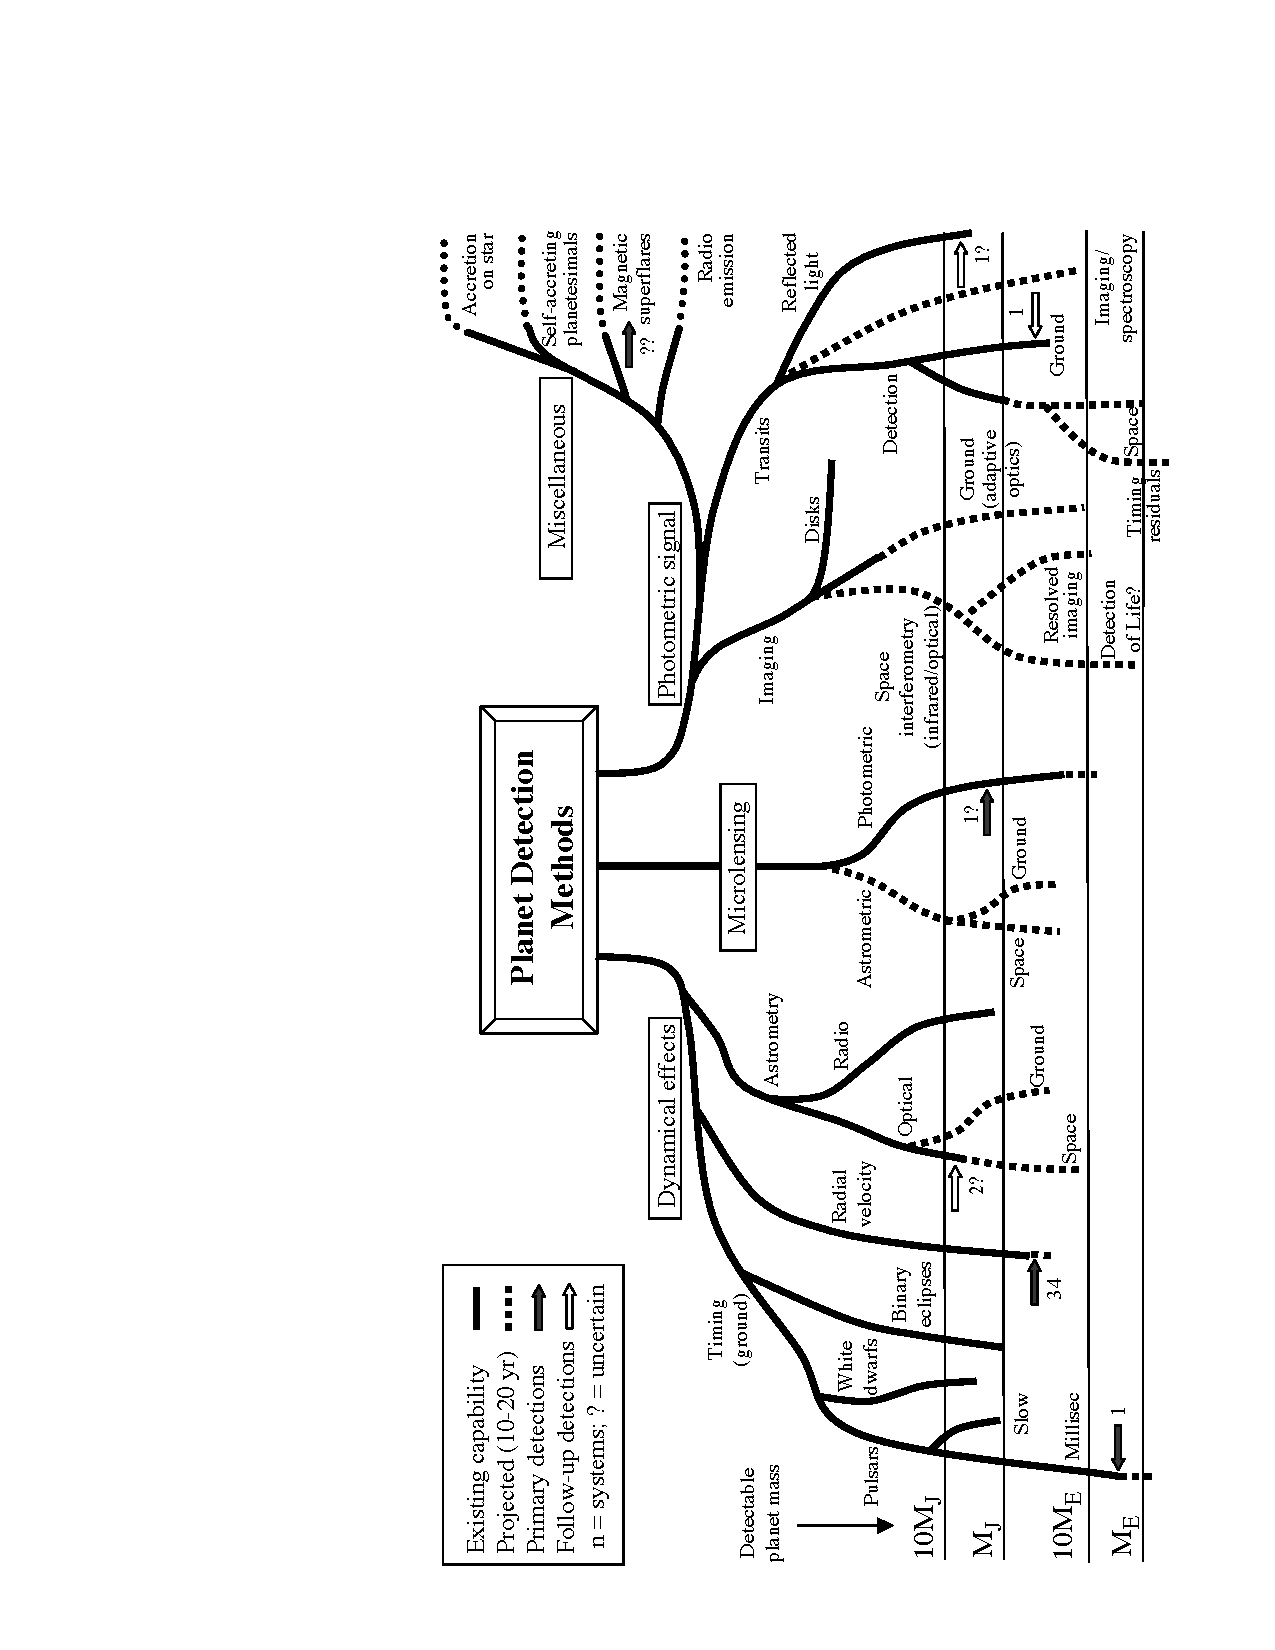
\includegraphics[scale=0.95, angle=-90]{figures/chapter1/fig4_fmethods.pdf}
    \caption[系外行星探测方法大全,图片版权 Michael Perryman。]{系外行星探测方法大全,关于图片说明请参见文献\citen{Perryman2000},此图摘录自该文献的第一幅插图。}
    \label{fig:detmethod}
\end{sidewaysfigure}


\section{行星形成理论} \label{sec:pltfrmatntheory}


星际空间并不是空无一物的,英国天文学家 William Herchel 在 18 世纪末观测到恒星周围冷暗物质
吸收带,我们的原太阳就是在这般空间环境中孕育而成\cite{Spitzer1978}。随着原初分子云坍缩,
核心区域会演化成原恒星,而周围的物质会由于原初角动量守恒而沉降成盘状结构以及双极喷流
(Bipolar Jets),比如观测到的 Herbig-Haro 型天体\cite{Lequeux2005}。

在恒星形成的早期,现有的观测证据主要集中在 T-Tauri 型天体上(又叫 Young Stellar Objects,
简称 YSOs)。YSOs 通常会按照红外谱指数($\alpha_\tif{IR} = \d\log \lambda F_\lambda)/(\d\log \lambda$)
分为 Class 0,Class \RN{1}, Class \RN{2}, Class \RN{3} 四种类型\cite{Andreetal2000}(见图
 \ref{fig:ysostage}),它们恰恰各自对应着不同的原恒星演化阶段。

\begin{figure}[b]
\centering
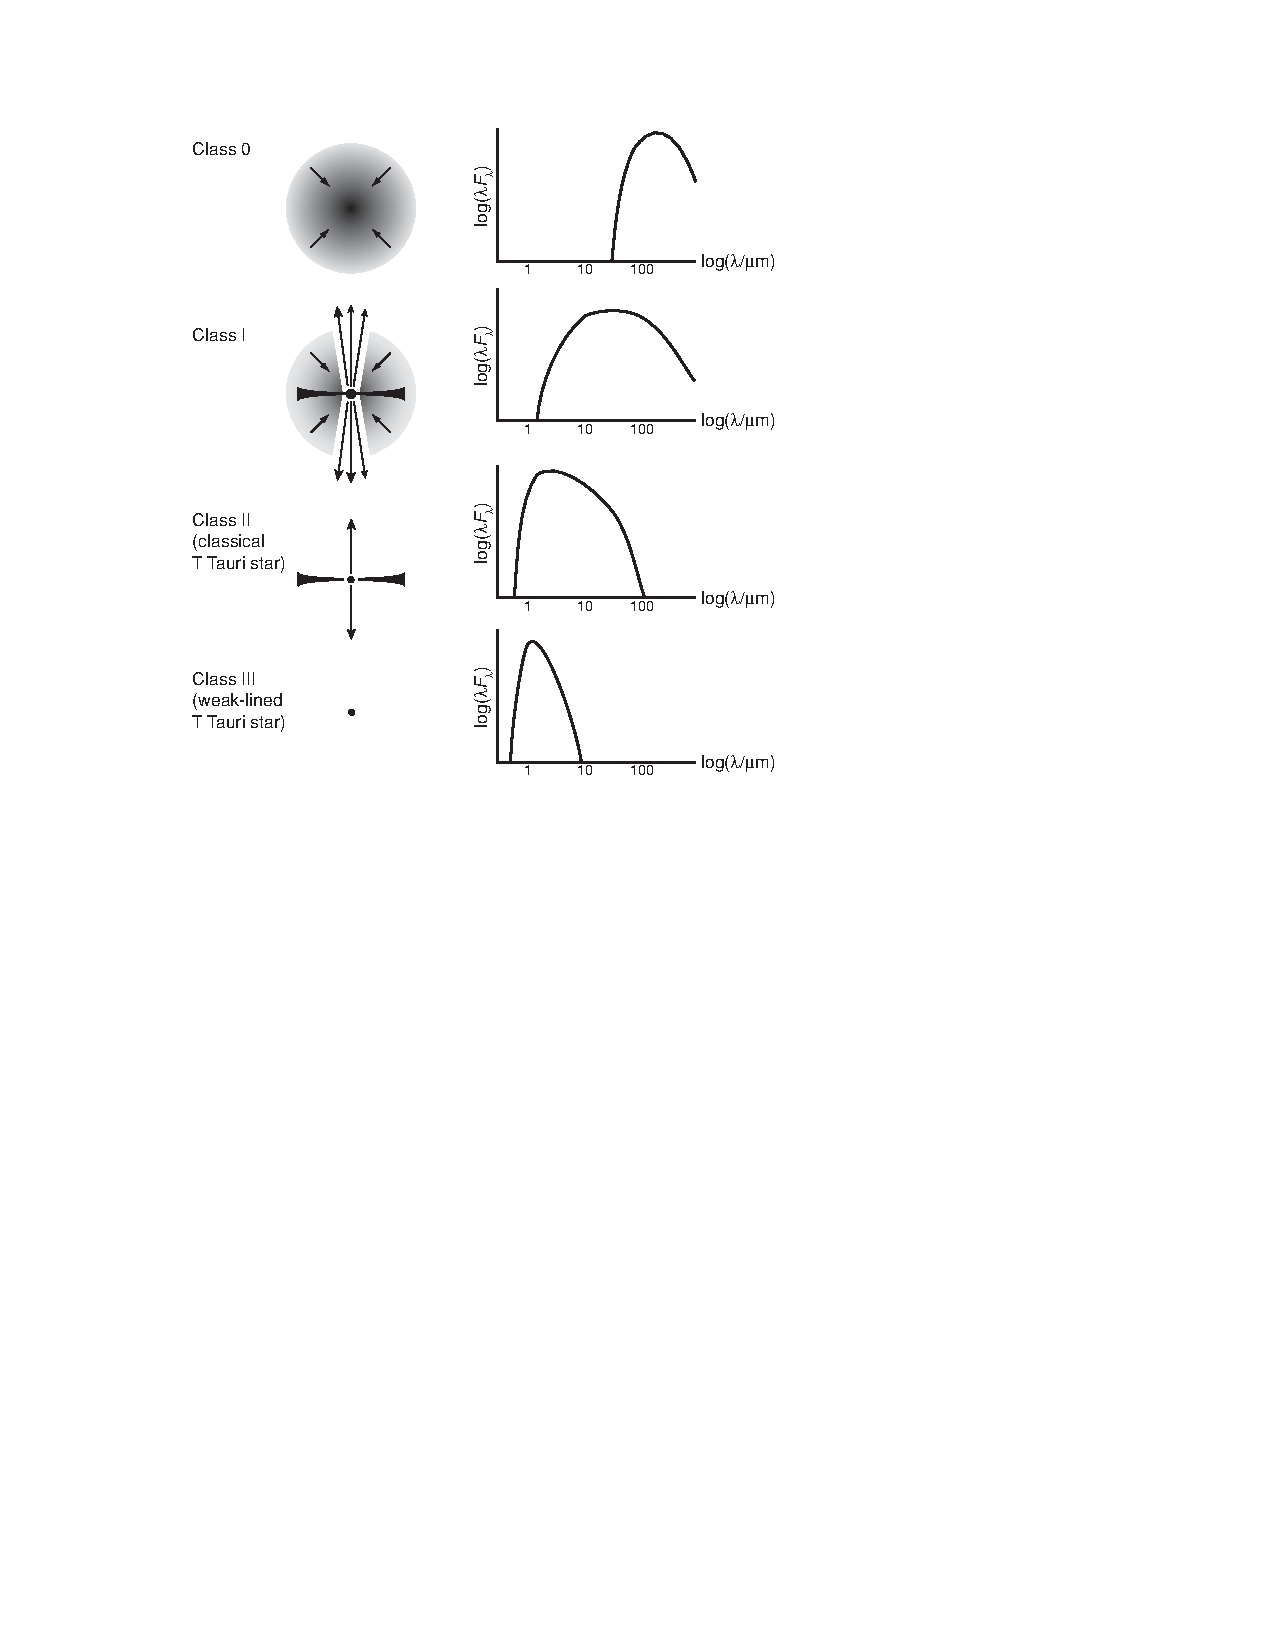
\includegraphics[width=0.95\textwidth]{figures/chapter1/fig9_ysostages.pdf}
\caption[YSOs 按照红外谱指数划分的四种主要类别,版权所有:Armitage P.。]{YSOs 按照红外谱指数划分的四种主要类别,图中背离黑体谱的红外突起部分又被称作红外超,它也是恒星是否存在盘的重要判据之一。此图取自书籍 \citen{Armitage2010}。}
\label{fig:ysostage}
\end{figure}

从某种程度上说,此刻的原恒星盘(Protostellar Disk)已可被称作原行星盘
\footnote{一般而言在恒星形成的早期,当恒星处于活跃吸积阶段时星周盘被称作原恒星盘,而在随后的行
星形成阶段则被称作原行星盘。}(Protoplanetary Disk)。根据文献\citen{Armitage2007},由于恒星对周
围气体的吸积\cite{Pringle1981}、恒星的高能辐射\cite{Johnstone1998,Hollenbach1994},以及气体
盘自身的粘滞性\cite{Shakura1973,Gammie1996},角动量会从从气体盘的内侧向外转移,原行星盘也会
逐渐耗散。2001 年,Haisch 等人通过统计不同星团中的红外超恒星比例,发现原行星盘的存活时标在不到
百万年(~10 Myr)的量级\cite{Haisch2001}。这对类木行星行形成有着非常重要的限制,因为木星必须在
气体盘消散前吸收足够的气体来长成如今的质量大小\cite{WilliamsCieza2011}。

\begin{figure}[t]
\centering
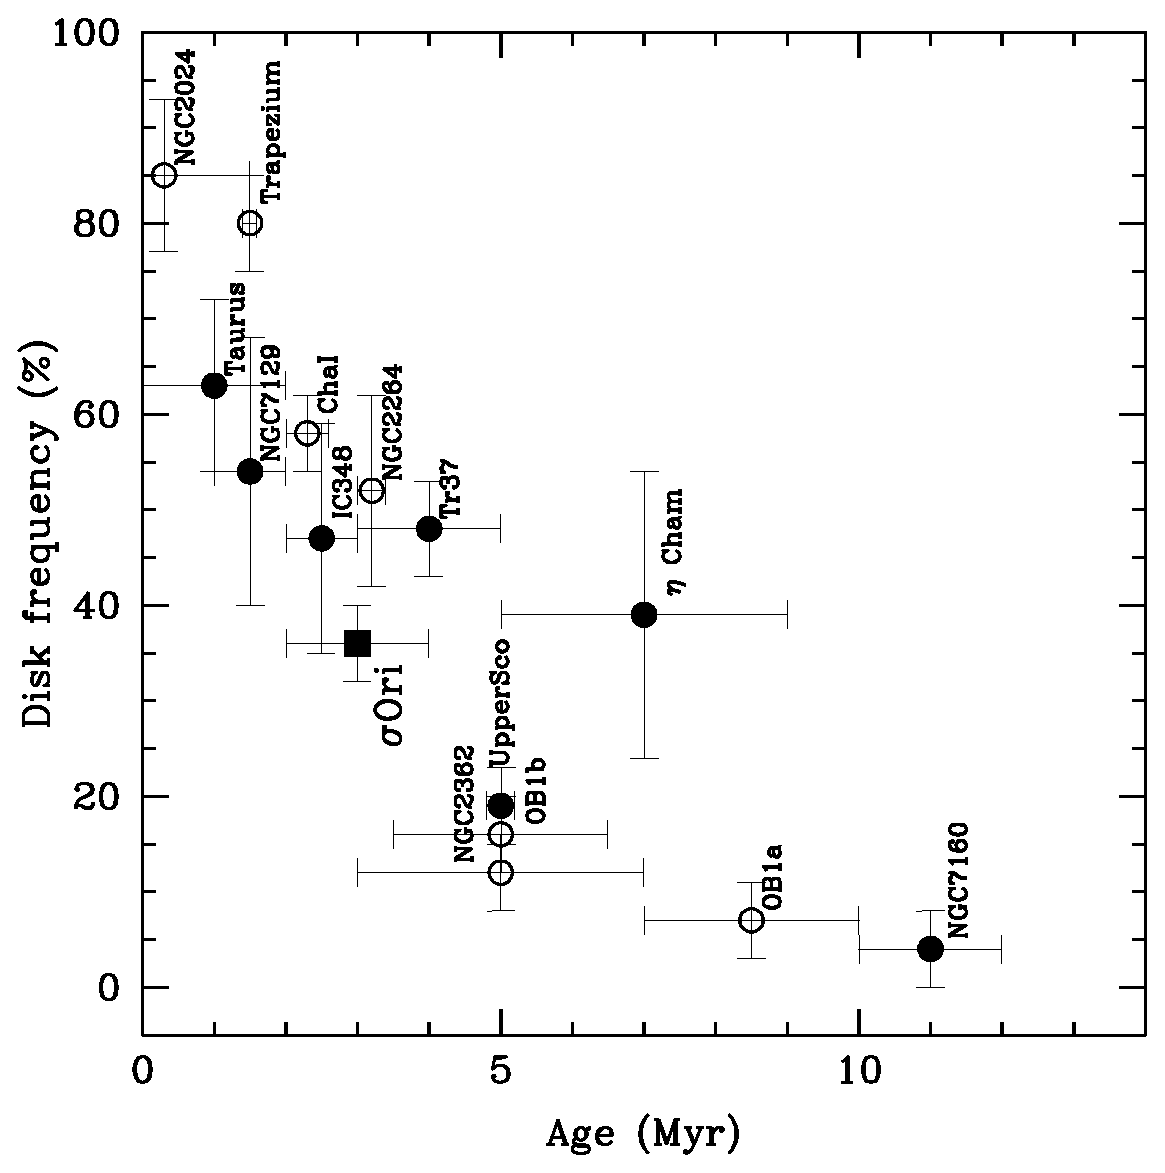
\includegraphics[width=0.95\textwidth]{figures/chapter1/fig10_pftimescale.eps}
\caption[不同星团红外超等效的原(恒)行星盘站所有星团成员的比例。此图可推断星团年龄老于10 Myr 后,恒星周围的气体盘已近乎完全消散。此图版权所有:Hern{\'a}ndez J. 等人。]{不同星团红外超等效的原(恒)行星盘站所有星团成员的比例。此图可推断星团年龄在 5 Myr 左右,恒星周围的气体盘已近乎消散。此图取自文献 \citen{Hernandez2007}。}
\label{fig:ysostage}
\end{figure}

\subsection{基于太阳系的经典行星形成理论} \label{sec:clspftheory}

早在 18 世纪中页,关于行星形成假说就已纷繁多样。其中康德、拉普拉斯等人提出的「星云假说」因
可较好应用至太阳系行星系统中而发展壮大。表\ref{tbl:solarsystem} 给出了太阳系八大行星的物理参数,
由此表可得出太阳系各大行星具有非常好的一致共面性,且除了水星以外都处于近圆轨道。如果将每个
行星的重元素平均到打散至行星之间的空隙中,并且混入适量的氢、氦使得新的混合物拥有与太阳相等
的金属丰度\footnote{在天文学中,金属元素特指氢和氦以外的所有重元素。}([Fe/H]),这样得到的最
小质量原太阳行星盘被称作 Minimum Solar Mass Nebula\cite{Weidenschilling1977,Hayashi1981},
MMSN 气体盘的面密度拥有如下的幂率函数形式:

\begin{equation} \label{eq:mmsng}
\Sigma_g = 1.7 \,\times10^3 \, \bigg(\frac{r}{\tif{AU}}\bigg)^{-3/2}  \tif{g} \,\tif{cm}^{-2}
\end{equation} %\myequation{最小质量太阳星云气体面密度分布表达式}

相应的固体盘的面密度分布同样可描述为:

\begin{equation} \label{eq:mmsns}
\Sigma_s = 7.1 \, f_\tif{ice} \, \bigg(\frac{r}{\tif{AU}}\bigg)^{-3/2}  \tif{g} \,\tif{cm}^{-2}
\end{equation} %\myequation{最小质量太阳星云固体面密度分布表达式}

其中 $f_\tif{ice}$ 为雪线因子。在距离太阳 2.7 AU 以外,水分子等会凝结成冰雪等固体物质,因而此因
子会从 1 增加至约 4.2\cite{IdaLin2004}。从此最小太阳星云模型出发,假若在垂直方向上给它一个标高
使其变为三维盘,这就是经典太阳系行星形成模型的开端。根据文献 \citen{Dullemond2005},重元素物
质(以微米到厘米级尘埃形式存在)会最先开始在垂直方向上沉降到盘的中平面;紧接着固体物质
(Dust)开始碰撞结合\cite{ppvibook2014,Weidenschilling1997,BlumWurm2008}或引力坍缩
\cite{Safronov1972,GoldreichWard1973,YoudinShu2002,ChiangYoudin2010}成星子(Planetesimal)。

\begin{table}[t]
\centering
\caption{太阳系八大行星物理参数与轨道参数,轨道根素值依照 J2000 平赤道参考系,数据取自 NASA/JPL 网站。}
\label{tbl:solarsystem}
\begin{tabular}{cccccccc}
\hline \hline
  & $a$(AU) & $P$(days) & $M_\tif{p}$($M_\oplus$) &  $e$ &  $i$(deg) &  $R_\tif{p}$($R_\oplus$) & $\rho$(g cm$^{-3}$) \\ \hline
水星        &   0.3871    &   88.0      &  0.0553    & 0.2056  &  7.00    &   0.383   &   5.427      \\
金星        &   0.7233    &   224.7    &  0.815      & 0.0068  &  3.39    &   0.949   &   5.243      \\
地球        &   1.000      &   365.2     &  1            & 0.0167 &   0.00    &   1          &   5.514      \\
火星        &   1.524      &   687.0     &  0.107     & 0.0934 &   1.85    &   0.532   &   3.933      \\
木星        &   5.203      &   4331      &  317.8     & 0.0484  &  1.30    &   11.2     &   1.326      \\
土星        &    9.537     &   10,747   &  95.2       & 0.0539 &    2.49   &   9.45     &   0.687      \\
天王星     &   19.19     &    30,589   &  14.5       & 0.0473 &   0.77    &   4.01     &  1.271       \\
海王星     &   30.07     &    59,800   &  17.1       & 0.0086 &    1.77   &    3.88    &  1.638       \\
\hline \hline
\end{tabular}
\end{table}

在 MMSN 模型下,星子的半径大概为公里量级。这样大小的星子和尘埃性质不同,它可以脱离气体的阻尼
力并通过自引力保持其结构。此时星子相互之间的引力作用变得显著,它们会经过雪崩增长与寡头生长两个
时期成长为原行星\cite{Greenberg1978,Kokubo1996,Rafikov2003,Lissauer1993}。原行星(亦称做行星胚胎)
会在接下来分别演化成气态巨行星和类地行星,其中形成气态巨行星一般被认为通过核吸积模型(Core Accretion)
\cite{Mizuno1980,BodenheimerPollack1986},而类地行星则需要经历更多的动力学作用过程才能形成
\cite{Chambers1998}。

当然,行星形成也还存在很多问题与挑战,解释太阳系太行星还存在许多难关\cite{Walsh2011,Morbidelli2005},
数值模拟如 Nice 模型\cite{Gomes2005Nice}也并不能解释所有太阳系构型(尤其是水的来源\cite{Raymond2009}),
本文仅能作粗略介绍,图 \ref{fig:pfstage} 为上述经典形成模型的核心各阶段过程的总结。

\begin{figure}[t]
\centering
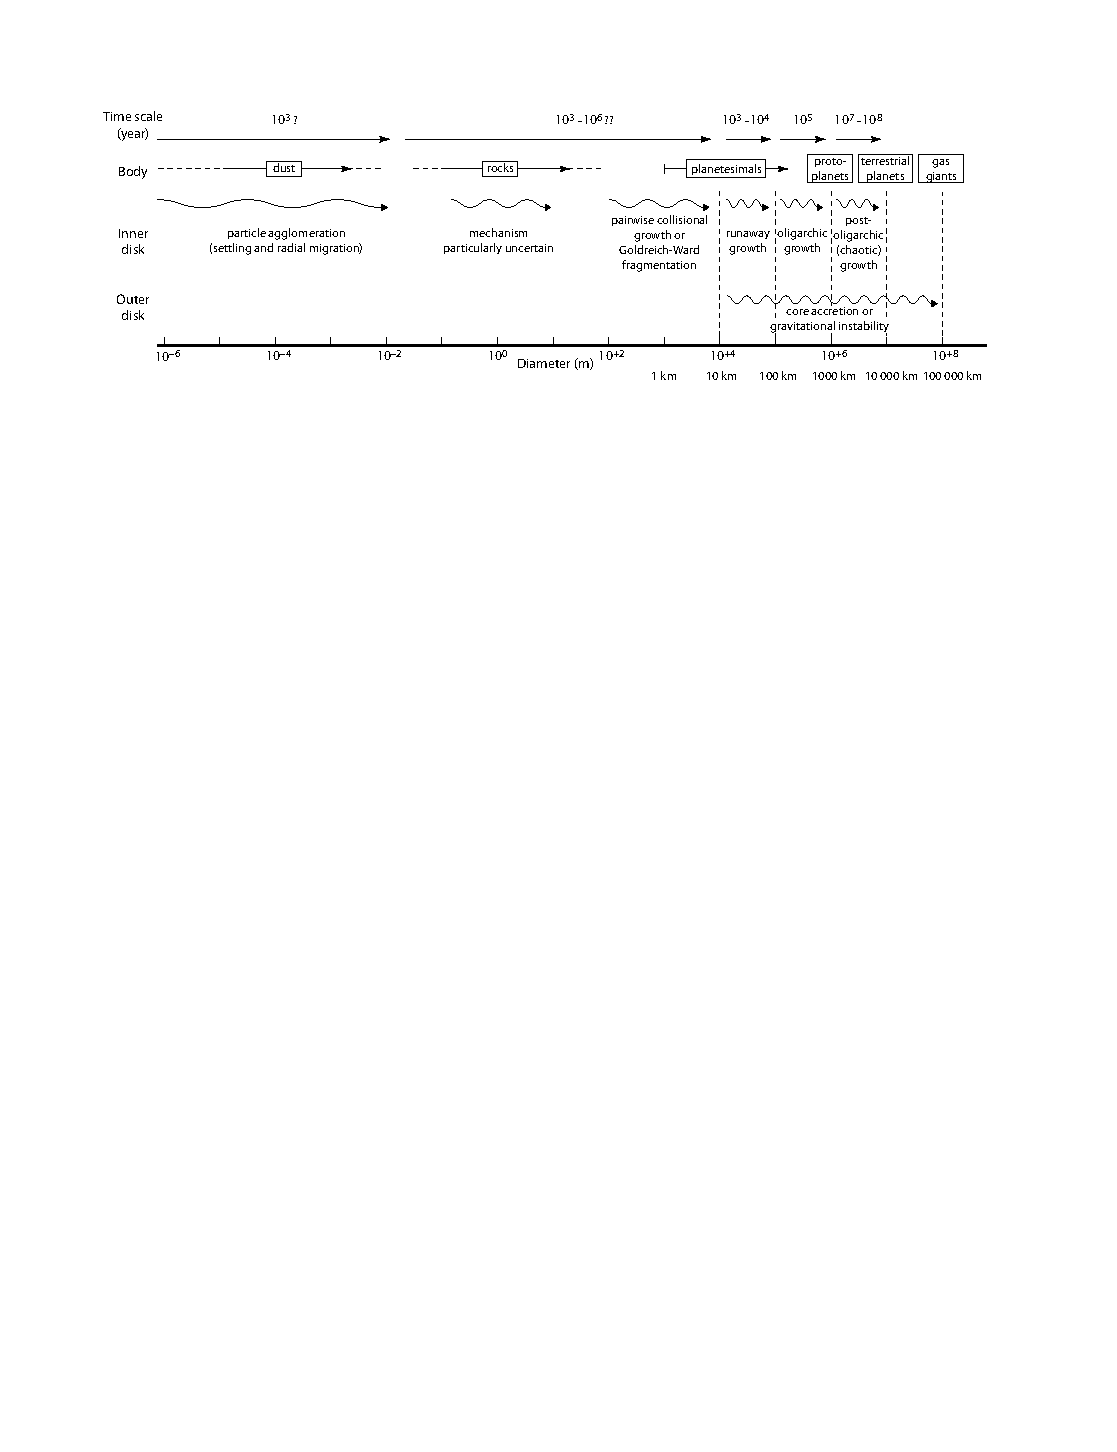
\includegraphics[width=1.0\textwidth]{figures/chapter1/fig11_pfsequence.pdf}
\caption[基于太阳系的传统行星形成理论模型在不同阶段的说明图,其中「米级障碍」属于至今为止的重大难题。图片版权 Michael Perryman。]{基于太阳系的传统行星形成理论模型在不同阶段的说明图,其中「米级障碍」属于至今为止的重大难题。此图取自文献 \citen{Perryman2014}。}
\label{fig:pfstage}
\end{figure}


\subsection{经典理论新挑战:系外行星} \label{sec: exopftheory}

百花齐放

热木星

Super Earth

单行星系统

多行星系统

主序后星周围

双星与星系团内

核坍缩

\section{本文立意}

